\chapter{Hypergraph Linguistic Model: Structure and Fusion}
\label{chap:ling_net}
\begin{abstractchap}
We present in this chapter our model proposition to stock linguistic data. This structure, based on the concept of hypergraphs, holds heterogeneous textual features, improving on the limitations of common solutions of the state of the art. At the same time, our network allows for fast access to words and their properties from different points of view. Finally, we also discuss our motivations and the scope and limitations of the network. 
\end{abstractchap}
\minitoc

\begin{figure}
\centering
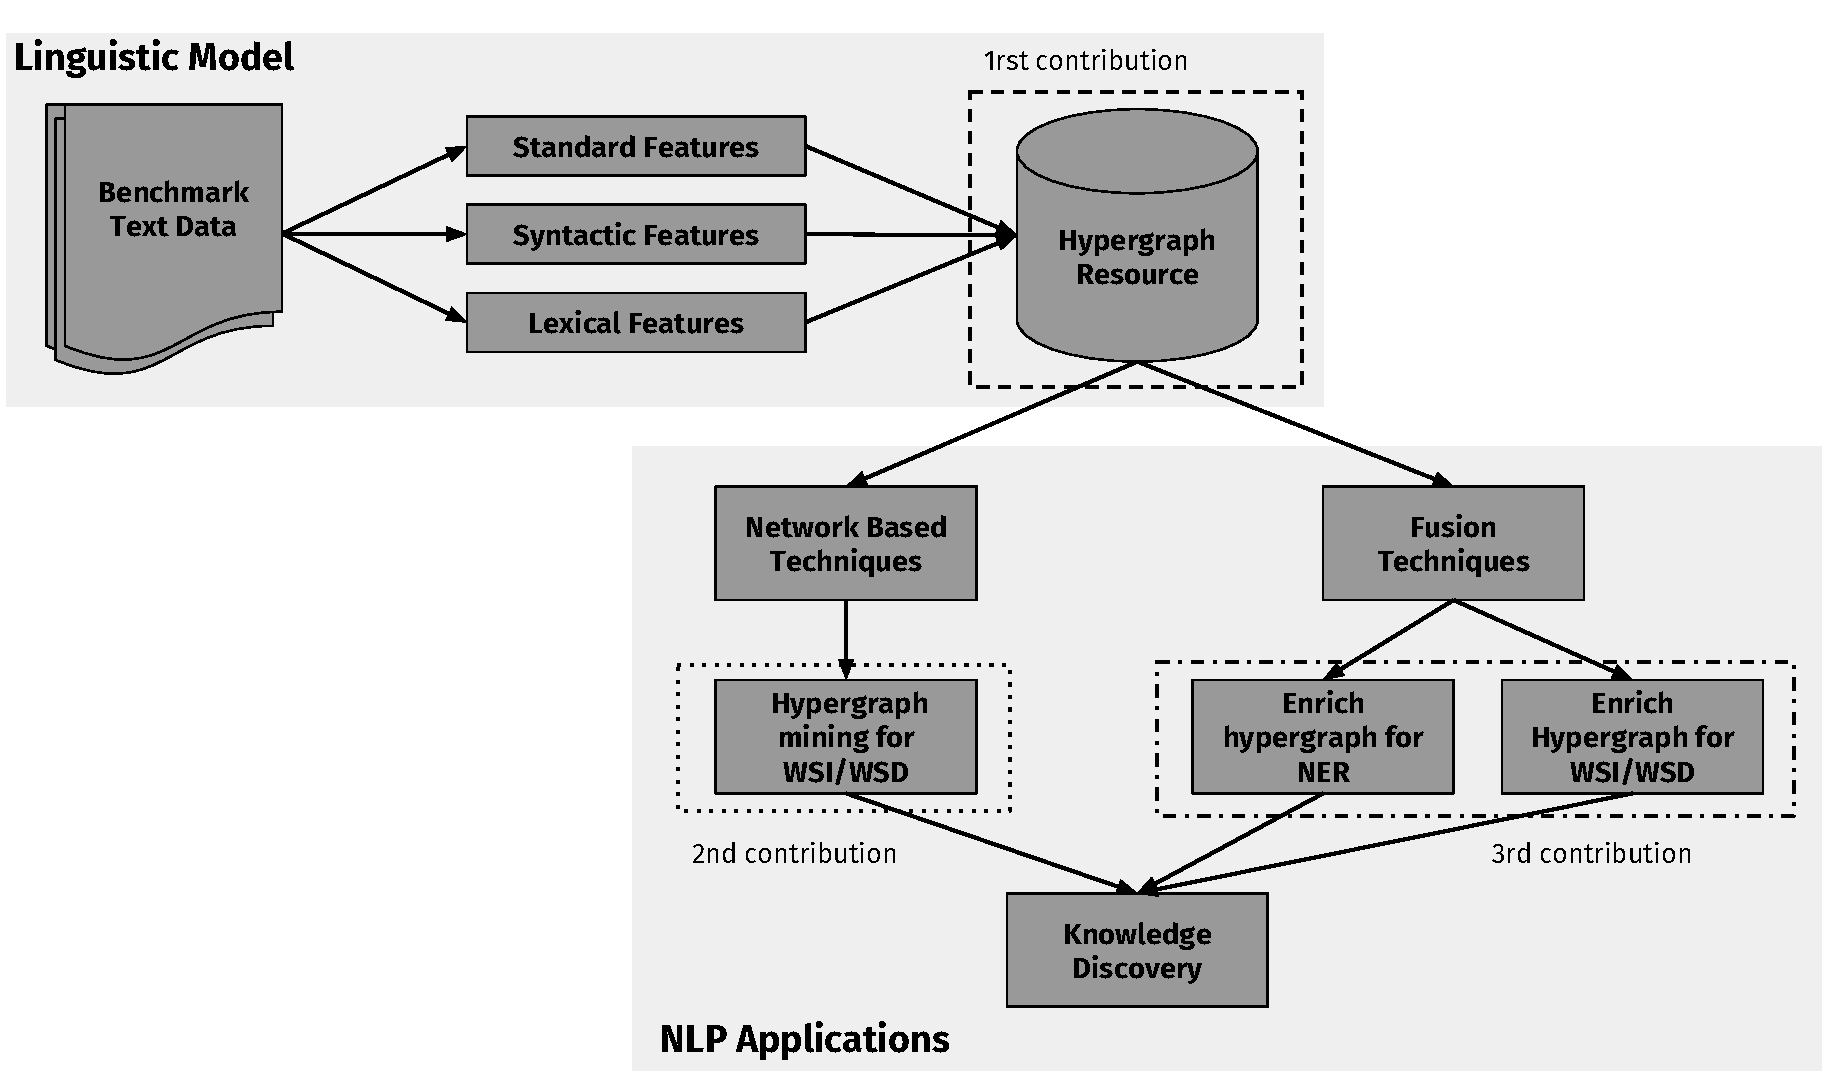
\includegraphics[width=1\linewidth]{./images/Chapitre3/main_diag.pdf}
\caption{Modular description of this dissertation}
\label{fig:maindiag}
\end{figure}

\section{Linguistic Networks}



In this chapter, we present an overview of linguistic network's related work. We first categorize them by their objectives and then by the data contained within. Next, we discuss what and how different methods are used with language networks to extract knowledge from their structural properties. Finally, we discuss the limitations of the current propositions and the advantages of the model we introduce in the following chapter.
%\minitoc
\subsection{Types of Linguistic Networks}

According to their objectives, we can consider two types of contributions in the linguistic-network literature: on the one hand, there are those approaches that investigate the nature of language via its graph representation, and on the other hand, we find those that propose a practical solution to a given NLP problem  \cite{Choudhury2009}. In particular, we pay attention to two aspects of a given network-based technique: (1) the  characteristics of the linguistic data within the network, and (2), the  algorithms used to extract knowledge from it.


In the following paragraphs we introduce the general categories of LNs according to their type of content and relations. We will introduce these categories as well as the  approaches that make use of them.

\cite{Mihalcea2011} defines four types of Language Networks (LN): co-occurrence network, syntactic-dependency network, semantic network and similarity network. Meanwhile, from a deeper linguistic point of view, \cite{Choudhury2009} introduces broader network's categories, each having several sub-types. The main difference (in our context) between both definitions lies in the separation of categories. In \cite{Choudhury2009}, they conflate syntactic-dependency and co-occurrence networks into the same  category: word co-occurrence networks. Similarly, they join semantic and similarity networks together and place them inside a broader category of lexical networks. The third  family  defined concerns phonological networks which is out of the scope of this work. In this work we will explore four categories of linguistic networks: semantic, lexical co-occurrence, syntactic co-occurrence and heterogeneous networks. The following sections will elucidate what each kind of network represent, we will mention works that employ this kind of networks and also list the main methodology differences that  variate from one approach to another. 
%These difference will be developed in subsection \ref{} and \ref{} where we discuss the nature of the language network graph as well as the algorithms used to obtain a practical solution to a NLP task.

\paragraph{Semantic Networks}
A Semantic Network (SN) relates words, or concepts, according to their meaning. The classical example of a SN is the renowned knowledge base Wordnet. This network, which serves also as an ontology, contains sets of synonyms (called synsets) as vertices and semantic relations as their edges. Typical semantic relationships include synonymmy-antnonimy, hypernym-hyponym, holonym-meronym. However, other semantic similarities can be defined. The edges are usually not weighted, although in some cases certain graph similarity measures may be used.

Word sense induction is indeed a task usually solved using semantic networks, specially Wordnet (and to a lesser extent, BabelNet) \cite{2004.Mihalcea.SemanticNetworkPageRank,2007.Sinha.Mihalcea.Unsupervised,2007.Tsatsaronis.WSDwithSpreading,2007.Navigli.GraphConnectivity,2008.Agirre.Multilingual,2008.Klapaftis.WSIUsingCollocations,2009.Agirre.PersonalizedPageRankWSD,2010.Klapaftis.WSD.WSD.HierarchicalGraphs,2010.Siberer.GraphCooccurrenceWSD,2014.Moro.Navigli.EntityLinking_WSD}. Given an input text with a set of ambiguous target words to process, these approaches follow a two-step algorithm:
\begin{enumerate}
\item Link target words (usually nouns, skipping stop-words and functional words) with their corresponding  sense (or synset in the case of WordNet-like dictionaries) and extract their vertices and edges into a new, smaller, SN. 
\item Apply a node ranking technique, usually a random-walk-based method, and select, for each ambiguous word in the input text,  its top ranking synset node as the correct sense.
\end{enumerate}

The amount of edges a SN has grows depending of the size of the version of Wordnet used or the level of polysemy of a given word. In order to avoid redundancy or contradiction between  linking nodes, \cite{2004.Mihalcea.SemanticNetworkPageRank,2007.Navigli.GraphConnectivity} applied pruning techniques to avoid \textit{contamination} while calculating ranking metrics in order to define a pertinent sense. Regarding edge similarity measures,  in  \cite{2007.Sinha.Mihalcea.Unsupervised, 2007.Tsatsaronis.WSDwithSpreading} they test some metrics individually and also combined. They found that the best results are indeed obtained when several metrics are used at the same time.

Other semantic tasks can also be solved using a SN. For example, Entity linking \cite{2014.Moro.Navigli.EntityLinking_WSD}. In their work, they leverage the BabelNet LKB to jointly disambiguate and link polysemous words to Wikipedia articles. 

Concerning the measure of semantic affinity between two terms, in \cite{2009.Yeh.Wikiwalk} they quantify word similarity by means of projecting them into a Wikipedia space. First, they represent each word by a vector representing its most pertinent pages,  and then they calculate a vectorial similarity measure between them.

In \cite{2013.Matuschek.Gurevych.Dijsktra.WSA} they propose a technique that aligns SNs, i.e., they link senses from two different networks. This task is called word sense alignment. Several SNs are used (Wordnet, Wikipedia, Wiktionary, etc.) thus nodes can represent synsets, articles, or concepts. The links may depict semantic relations or may be links joining two concepts or pages together. Their approach aims to find the shortest path between nodes of any two given SNs while leveraging already existing links between  equal concepts found in both SNs.



Finally, extracting entities from text can also benefit from the use of SNs. The work proposed by  \cite{2013.Kivimaki.AGraph-BasedApproach} aims to extract technical skills from a document. Again, using Wikipedia as SN, they first represent each article and the input document in a token vector space model.  Next, they find the document top 200 similar pages by calculating the cosine similarity between the document and each page. This serves to extract a Wikipedia subgraph which is used to calculate the most relevant pages for the entry document. Finally, the top pages are filtered by means of selecting those articles that actually represent a skill using a fixed list of skill-related tokens. Once again, the nodes represent Wikipedia articles and the edges the hyperlinks that join them.


The cited methods vary in how they make use of their SN, not so much in the network per se. These differences boil down to three aspects:
\begin{bulletList}
\item Type of relationship implied by the edges linking the nodes of the network, 
\item The algorithm used to rank the nodes after the semantic network is built, and
\item The weight assigned to each edge.
\end{bulletList}


\paragraph{Lexical Co-occurrence Networks}
Most co-occurrence based intuitions in NLP have their origin in the distributional hypothesis. An effective way to  represent word co-occurrences is by means of a graph structure. Indeed, this kind of graphs are the central column of a Lexical Co-occurrence Network (LCN). In these structures, nodes represent words and edges indicate co-occurrence between them, i.e., two words appear together in the same context. A context can vary from a couple of words (before or after a given word) to a full document, although it is usually defined at sentence level. The edges' weight  represent the strength of a link and is generally a frequency based metric that takes into account the  number of apparitions of each word independently and together.

To solve a task in a truly unsupervised way, researchers generally use this kind of networks instead of LKBs. It is then natural that word sense disambiguation approaches leverage lexical co-occurrence networks, and in return, the distributional hypothesis, to automatically discover senses for a given target word. That is why WSI methods \cite{2004.Veronis,2007.Klapaftis.UOY,2010.Navigli.InducingWordSenses.Triangles,2008.Klapaftis.WSIUsingCollocations,2011.DiMarco.Navigli.ClusteringWebSearch,2011.Jurgens.WSICommunityDetection} are tightly related to LCNs. 
The cited works use a LCN as described before while other works such as \cite{2007.Navigli.GraphConnectivity,2014.Tao.Qian.LexicalChainHypergraphWSI} represent the co-occurrence by means of a hypergraph scheme. In short, a hypergraph structure is a graph generalization where an edge (called hyperedge) can link more than two vertices per edge and thus it is able to provide a more complete description of the interaction between several nodes \cite{estrada2005}.

In their paper, given an input document with several contexts for each target word, they first group together the contexts via a topic-modeling technique. Thus, each context is assigned a particular group (in this case, a topic). Secondly, a hypergraph is built where the vertices represent contexts and the hyperedges link two nodes together if they share the same topic. Thirdly, the hypergraph is clustered and the words of each context (of each node) are used to build vectorial representations

WSI systems generally perform four steps. Given an input text with a set of target words and their contexts (target words must have several instances throughout the document to cluster them), the steps are the following:

\begin{enumerate}
\item Build a LCN, assigning tokens as nodes and  establishing edges between them if they co-occur in a given context (usually if they both appear in the same sentence),
\item Determine the weights for each edge according to a frequency metric,
\item Apply a graph clustering algorithm. Each cluster found will represent a sense of the polysemous word, and
\item Match  target word instances with the clusters found by leveraging each target word context. Specifically, assign a cluster (a sense) to each instance by looking at the tokens in the context.
\end{enumerate}

As with semantic networks, not only WSD or WSI can be solved with LCNs. Finding semantic associated terms in a corpus is a critical step in several NLP systems. This task is solved in the system proposed by \cite{2011.Haishan.AHypergraphbased}. They also use a LCN although instead of a co-occurrence graph, they also employ a co-occurrence hypergraph, where nodes represent words and edges describe co-occurrence at the paragraph level.  In this work, they use such structure to find related terms in a given corpus. In order to do it, they mine the hypergraph as in a frequent itemsets problem, where the items are the words from a text. The method consists in first finding similar itemsets by means of measuring similarity between nodes. Once the 2-itemsets are found, they induce a graph from the original hypergraph by drawing edges between nodes that have a similarity superior to an arbitrary threshold. Lastly, in order to find $k$-itemsets ($k > 2$), the find either complete or connected components in the induced graph. 



As with WSD, while the LCNs used are mostly the same among approaches, there are certain moving parts that make up the difference between WSI approaches. The most common differences that can arise are:

\begin{itemize}
\item The clustering algorithm to find senses in the LCN graph.
\item The technique used to match context words to clusters.
\item The weight used in the graph edges.
\end{itemize}



\paragraph{Syntactic Co-occurrence Networks}
A Syntactic Co-occurrence Network (SCN) is very similar to a LCN  in the sense that both exploit the distributional hypothesis. Nonetheless, SCNs go further by leveraging  syntactic information extracted from the text. There are two main types of syntactic information both represented as tree structures: constituency-based parse trees and dependency-based parse trees. Briefly, the former structure splits a phrase into several sub-phrases. In this way we can get a glimpse of the role of each word inside a phrase. The latter tells us about the relationships existing between words in the phrase. SCNs employ, most of the time, dependency trees to create a graph that relates words according to their syntactic relations. In the case of \cite{2013.Hope.GradedWSI}, a graph is built using syntactic dependencies. It is used to perform WSI using a very similar approach as those systems using LCNs. 

A network representation that is on the border line between being a LCN and a SCN is that of \cite{2013.Bronselaer.TextAnalysisWithGraphs}. They  propose a graph document modelization. In their network, nodes represent words and edges their co-occurrence, as any LCN. Still, their graph resembles a SCN because the edges may represent one of three types of words: either prepositions, conjunctions or verbs. As a result,  they need to first extract syntactic information from a document, namely the part-of-speech tags of each word. They find the most relevant words of a given text by ranking the nodes of the graph. The words that best represent a document can be used to summarize it, as they show in their work.

Approaches based on SCN are rarely used in WSD or WSI systems, and therefore they are an interesting research avenue to explore.


\paragraph{Heterogeneous Networks}
Until now we have described different types of networks with single types of nodes and relations. Lately, heterogeneous networks have been defined in order to model multi-typed information in a single structure \cite{Jiawei2009}. 

Even though this kind of structure seems to open new avenues of research in the semantic analysis domain, only few explicitly take advantage of them, as is the case of \cite{2013.Saluja.Graph-BasedUnsupervisedLearning}. In their approach, they build a graph that links together features with words, and discover similarity measures that leverage the multi-typed nature of their network.


\subsection{Algorithms used in Linguistic Networks}

We have discussed until now the different types of networks from a content point of view. In this subsection, we address the details of the algorithms used to solve practical NLP tasks. In this section we will cover the details of four different types of graph algorithms.

%\paragraph{Notation}
%In this section we will be referring to a connected undirected graph, which we denote by $G = (V,E,W)$. The graph $G$ has vertex set $V$, edge set $E$ where $|V|=n$, $|E|=m$, and the matrix $W\in\mathbb{R}^{n\times n}$, with $w_{u,v} \geq 0$, defines any kind of weights in the graph.


\paragraph{Edge Weights}

We begin by describing the metrics used to determine similarity between nodes, usually stored as edge weights. As stated in the previous sections, most of the metrics are frequency based, specially when dealing with LCNs. The main idea of these measures is to assign a weight that decreases as the association frequency of the words increases. Among these measures, the most popular are the Dice  coefficient \cite{2010.Navigli.InducingWordSenses.Triangles,2011.DiMarco.Navigli.ClusteringWebSearch,2013.DiMarco.Navigli.ClusteringGraph-BasedWSI}, normalized pointwise mutual information \cite{2013.Hope.GradedWSI}, and a graph-adapted tf-idf variant \cite{2007.Tsatsaronis.WSDwithSpreading} which aims to give importance to frequent edges while also favoring those that are rare.

Edge weights can also be calculated when the vertices of a network do not represent words. Such is the case of \cite{2010.Klapaftis.WSD.WSD.HierarchicalGraphs}, where nodes represents a target word context (set of tokens around an ambiguous word). This time the Jaccard index is used to quantify similarity between them while considering how many words are shared between a pair of context nodes.

%When the nodes represent synsets (or concepts), certain approaches leverage only the intrinsic nature of the network connections, leveraged by random walk algorithms, without explicitly using  weighted edges \cite{2004.Mihalcea.SemanticNetworkPageRank}. 
% On the other hand, there are techniques that assign a frequency-based weight to represent the importance of a semantic relation, particularly those found in the reviews  by \cite{2007.Sinha.Mihalcea.Unsupervised,2007.Navigli.GraphConnectivity}, where several weights are tested.

A  more sophisticated approach to edge weighting is proposed in \cite{2013.Saluja.Graph-BasedUnsupervisedLearning} where they employ  custom-defined functions in order to learn the most appropriate edges' weights for a given set of seed vertices inside a network. The main idea  is to enforce \textit{smoothness} (keeping two nodes close if they have related edges) across the network.

As a way to rank edges according to their importance, the ratio of triangles (cycles of length 3), squares (cycles of length 4), and diamonds (graphs with 4 vertices and 5 edges, forming a square with a diagonal) in which an edge participates are calculated \cite{2010.Navigli.InducingWordSenses.Triangles,2013.DiMarco.Navigli.ClusteringGraph-BasedWSI}. Once the top edges are found, they create a subgraph containing only these edges (and its corresponding vertices).

Finally, instead of applying weights to edges, a case where  nodes are weighted can be found in \cite{2013.Kivimaki.AGraph-BasedApproach}. They measure and remove popular nodes in order to avoid their bias during the application of their random walk approach.




 

\paragraph{Graph Search}
Usually, in a WSD approach, the first step to follow is to build a graph from a LKB. The goal is to explore the semantic network and find all the senses linked to  those found in the context of an ambiguous word. Aside from custom search heuristics applied by certain works \cite{2006.Agirre.TwoGraph-basedAlgorithms,2007.Sinha.Mihalcea.Unsupervised,2009.Agirre.PersonalizedPageRankWSD}, researchers also use well-known graph techniques such as depth-first search \cite{2007.Navigli.GraphConnectivity}, breadth-first search \cite{2008.Agirre.Multilingual} and even the Dijsktra  algorithm to find the group of closest senses in the network \cite{2013.Matuschek.Gurevych.Dijsktra.WSA}.


\paragraph{Node Connectivity Measures}\label{sec:connectivity_measures}
A Connectivity Measure (CM) determines the importance of a node in a graph according to its association with other nodes. In most cases its value ranges from zero to one, where the 0 indicates that the node is of minor importance while 1 suggests a relatively high significance. Nowadays, the most widely used  measures are those based on random walks.

A Random Walk (RW) can be simply defined as the traversal of a graph beginning from a given node and randomly jumping to another in the next time step.
% It is similar to a Markov chain process, the difference being that in a Markov chain the next step node is chosen to according to a certain distribution.  

PageRank \cite{Brin1998}, the popular random walk based algorithm is used commonly in WSD. The recursive intuition of PageRank is to give importance to a node according to the PageRank value of the nodes that are connected to it. %Formally, the vector PageRank holding values for each node in $v \in V$ is calculated as: $PR(v) = \alpha\sum_{u,v\in E}{\frac{PR(u)}{outdegree(u}} + \mathbf{v}(1-\alpha)$, where $ \alpha  $ is a dumping factor to control the jumps a random walker will make; and $ \mathbf{v} $ is the relevance vector for each node has in $G$. In classical PageRank, the values of  $\mathbf{v}$ are uniformly set to $\frac{1}{n}$ for all nodes in $|V|$. 
Nonetheless, as a regular random-walk algorithm, in PageRank the probability distribution to change from a node to another is uniform. In such case, the jumps a random walker performs depend solely on the nature of the graph studied. Among the approaches surveyed, those that use the most PageRank are those that solve word sense disambiguation \cite{2004.Mihalcea.SemanticNetworkPageRank,2006.Agirre.TwoGraph-basedAlgorithms,2007.Navigli.GraphConnectivity,2010.Siberer.GraphCooccurrenceWSD}. 
%
These approaches make a conventional use of PageRank: they apply it and rank nodes to select the most appropriate senses for ambiguous words. Still, there are some improvements over the classical use of PageRank in WSD. Some techniques employ a different version of PageRank called Personalized PageRank (or PageRank with restart \cite{Murphy2012} or PPR) were a random walker may return to a specific starting node with certain probability rather than jumping to a random node. This formulation allows researchers to assign more weight to certain nodes. For example, in \cite{2009.Agirre.PersonalizedPageRankWSD} they are able to use the complete Wordnet graph as their SN. They do this by directly adding context words of a polysemous token into Wordnet and then giving a uniform initial distribution to only these nodes. In this way, they force PageRank to give more importance to the context words without the need of extracting a subgraph from the SN. In \cite{2014.Moro.Navigli.EntityLinking_WSD} they apply the same technique to obtain a \textit{semantic signature} of a given sense vertex. After applying PPR, they obtain a frequency distribution over all the  nodes in the graph. The so-called semantic signature consists in those nodes that were visited more than an arbitrary threshold and that best represent an input sense node.

There are other methods which share the properties of random walk approaches. In  \cite{2007.Tsatsaronis.WSDwithSpreading,2013.Kivimaki.AGraph-BasedApproach} they apply a method known as spreading activation. This algorithm aims to iteratively diffuse the initial weights of a set of seed nodes across the network. Specifically, once a weighted semantic network is built, they \textit{activate}  the nodes representing the context senses, assigning a value of 1, while \textit{disactivating} the rest by setting them to 0. They determine the most pertinent senses to the input nodes by storing, for each of them, the last active sense node with the highest activation value. 

Beyond WSD and into the task of determining word similarities, we found the work of \cite{2009.Yeh.Wikiwalk}, where they calculate a semantic similarity between a pair of words while leveraging a Wikipedia SN. For each word, they  apply PPR to find the articles that best represent a word. 
%They set the initial distribution in such a way that the articles that best represent each word have a higher probability than the rest of nodes. 
In \cite{2013.Saluja.Graph-BasedUnsupervisedLearning}, they also employ PPR to find synonym words given a word-similarity matrix and a new unknown word (also known as out-of-vocabulary word). They link the new word to its corresponding feature nodes and they normalize the similarity matrix to use the weights as probabilities and thus bias the random walk. In \cite{2013.Kivimaki.AGraph-BasedApproach} they use centrality measures to determine the most relevant nodes in a SN and then, in contrast with most approaches, remove them from the graph in order to not bias their graph algorithms.
%

With regard to other CMs, there are  more elementary alternatives to determine the importance of a node. For example, the approaches of  \cite{2004.Veronis,2007.Klapaftis.UOY,2011.Haishan.AHypergraphbased,2013.Bronselaer.TextAnalysisWithGraphs,2014.Moro.Navigli.EntityLinking_WSD} successfully use the degree of a node, or other metric, to determine its importance in a network.






\paragraph{Graph Clustering/Partitioning}

Graph clustering is defined as the task of grouping the vertices of a graph into clusters while taking into consideration its edge structure \cite{Schaeffer2007}. As previously mentioned, graph-based word sense induction relies most importantly in the graph clustering step where the actual senses of a word are inferred. 

In this subsection we also consider  subgraph extracting techniques which are exploited to find separated groups of words and thus induce senses. In this context we found the approaches of \cite{2004.Veronis,2010.Siberer.GraphCooccurrenceWSD}. These systems make use of both the Minimum and Maximum Spanning Trees algorithms (MinST and MaxST, respectively) as a final step to  disambiguate a target word given its context.  Meanwhile, both \cite{2011.Haishan.AHypergraphbased,2014.Tao.Qian.LexicalChainHypergraphWSI}  use the Hypergraph Normalized Cut (HCT) approach, a hypergraph clustering method based on minimum cuts, to induce senses.

Most of the reviewed approaches employ state of the art techniques \cite{2008.Klapaftis.WSIUsingCollocations,2010.Klapaftis.WSD.WSD.HierarchicalGraphs,2011.Jurgens.WSICommunityDetection,2013.Hope.GradedWSI}. Specifically, they utilize Chinese Whispers (CW) \cite{biemann2006chinese}, Hierarchical Random Graphs (HRG) \cite{clauset2008hierarchical}, Link Clustering (LC) \cite{ahn2010link}, and MaxMax (MM) \cite{hope2013maxmax} respectively. 

Briefly, CW is a randomized graph-clustering method  which is time-linear with respect to the number of edges and does not need a fixed number of clusters as input. It only requires a maximum amount of iterations to perform. HRG, being a hierarchical clustering algorithm, groups words into a binary tree representation, which allows to have more in-detail information about the similarity among words when compared to flat clustering algorithms. Regarding LC, instead of clustering nodes, this procedure groups edges. Thus it can identify contexts related to certain senses, instead of finding groups of words as most approaches do. Finally, MM, is able to assemble words into a fixed cluster (hard clustering) or allow them to be in several groups at the same time (soft clustering). It shares certain characteristics with CW:  they are both methods that exploit similarity within the local neighborhood of nodes and both are time-linear. Nonetheless, a key difference is that CW is not deterministic, while MM is, thus MM will find always the same clustering result for the same input graph.

 
 


\begin{table}[]
\centering
\caption{Survey summary table.}
\label{tab:survey_sum}
\setlength\tabcolsep{1.8mm}
\def\arraystretch{.95}%
\begin{tabular}{l|cccc|cccc}
\hline
\textbf{\textbf{Approach}}                                                       & \multicolumn{4}{c|}{\textbf{Network Type}}                                                                                                              & \multicolumn{4}{c}{\textbf{Algorithms}}                                                                                                                                                                                                                            \\ \hline
                                                                                 & \rotatebox[origin=c]{90}{Semantic} & \rotatebox[origin=c]{90}{Lexical} & \rotatebox[origin=c]{90}{Syntactic} & \rotatebox[origin=c]{90}{Heterogeneous} & \rotatebox[origin=c]{90}{Edge Wts.} & \rotatebox[origin=c]{90}{Graph Search} & \rotatebox[origin=c]{90}{Connectivity Meas.} & \rotatebox[origin=c]{90}{Graph Clust.} \\ \hline
Veronis, 2004 \cite{2004.Veronis}                                                &                                    & x                                 &                                     &                                         &                                                                                  &                                        & x                                               & x                                                                                    \\
Mihalcea et al., 2004 \cite{2004.Mihalcea.SemanticNetworkPageRank}               & x                                  &                                   &                                     &                                         &                                                                                  &                                        & x                                               &                                                                                      \\
Agirre et al., 2006 \cite{2006.Agirre.TwoGraph-basedAlgorithms}                  &                                    & x                                 &                                     &                                         &                                                                                  & x                                      & x                                               &                                                                                      \\
Sinha and Mihalcea, 2007 \cite{2007.Sinha.Mihalcea.Unsupervised}                 & x                                  &                                   &                                     &                                         &                                                                                  & x                                      &                                                 &                                                                                      \\
Navigli and Lapata, 2007\cite{2007.Navigli.GraphConnectivity}                    & x                                  &                                   &                                     &                                         &                                                                                  & x                                      & x                                               &                                                                                      \\
Tsatsaronis et al., 2007 \cite{2007.Tsatsaronis.WSDwithSpreading}                & x                                  &                                   &                                     &                                         &                                                                                  &                                        & x                                               &                                                                                      \\
Klapaftis and Manandhar, 2007 \cite{2007.Klapaftis.UoY}                          &                                    & x                                 &                                     &                                         & x                                                                                &                                        & x                                               &                                                                                      \\
Klapaftis and Manandhar, 2008 \cite{2008.Klapaftis.WSIUsingCollocations}         &                                    & x                                 &                                     &                                         & x                                                                                &                                        &                                                 & x                                                                                    \\
Agirre and Soroa, 2008 \cite{2008.Agirre.Multilingual}                           & x                                  &                                   &                                     &                                         &                                                                                  & x                                      &                                                 &                                                                                      \\
Agirre and Soroa, 2009 \cite{2009.Agirre.PersonalizedPageRankWSD}                & x                                  &                                   &                                     &                                         &                                                                                  & x                                      & x                                               &                                                                                      \\
Klapaftis and Manandhar, 2010 \cite{2010.Klapaftis.WSD.WSD.HierarchicalGraphs}   &                                    & x                                 &                                     &                                         & x                                                                                &                                        &                                                 & x                                                                                    \\
Navigli and Crisafulli, 2010 \cite{2010.Navigli.InducingWordSenses.Triangles}    &                                    & x                                 &                                     &                                         & x                                                                                &                                        &                                                 &                                                                                      \\
Silberer and Ponzetto, 2010 \cite{2010.Siberer.GraphCooccurrenceWSD}             &                                    & x                                 &                                     &                                         &                                                                                  &                                        & x                                               & x                                                                                    \\
Di Marco and Navigli, 2011 \cite{2011.DiMarco.Navigli.ClusteringWebSearch}       &                                    & x                                 &                                     &                                         & x                                                                                &                                        &                                                 &                                                                                      \\
Jurgens, 2011 \cite{2011.Jurgens.WSICommunityDetection}                          &                                    &                                   &                                     &                                         &                                                                                  &                                        &                                                 & x                                                                                    \\
Di Marco and Navigli, 2013 \cite{2013.DiMarco.Navigli.ClusteringGraph-BasedWSI}  &                                    & x                                 &                                     &                                         & x                                                                                &                                        &                                                 &                                                                                      \\
Hope and Keller, 2013 \cite{2013.Hope.GradedWSI}                                 &                                    &                                   & x                                   &                                         & x                                                                                &                                        &                                                 & x                                                                                    \\
Moro et al., 2014 \cite{2014.Moro.Navigli.EntityLinking_WSD}                     & x                                  &                                   &                                     &                                         &                                                                                  &                                        & x                                               &                                                                                      \\
Qian et al., 2014 \cite{2014.Tao.Qian.LexicalChainHypergraphWSI}                 & x                                  & x                                 &                                     &                                         &                                                                                  &                                        &                                                 & x                                                                                    \\
Yeh et al., 2009 \cite{2009.Yeh.Wikiwalk}                                        & x                                  &                                   &                                     &                                         &                                                                                  &                                        & x                                               &                                                                                      \\
Liu et al., 2011 \cite{2011.Haishan.AHypergraphbased}                            &                                    & x                                 &                                     &                                         &                                                                                  &                                        & x                                               & x                                                                                    \\
Matuschek and Gurevych, 2013 \cite{2013.Matuschek.Gurevych.Dijsktra.WSA}         & x                                  &                                   &                                     &                                         &                                                                                  & x                                      &                                                 &                                                                                      \\
Bronselaer and Pasi, 2013  \cite{2013.Bronselaer.TextAnalysisWithGraphs}         &                                    &                                   & x                                   &                                         &                                                                                  &                                        & x                                               &                                                                                      \\
Kivim\"{a}ki et al., 2013 \cite{2013.Kivimaki.AGraph-BasedApproach}              & x                                  &                                   &                                     &                                         & x                                                                                &                                        & x                                               &                                                                                      \\
Saluja and Navr\'{a}til, 2013 \cite{2013.Saluja.Graph-BasedUnsupervisedLearning} &                                    & x                                 &                                     & x                                       & x                                                                                &                                        & x                                               &                                                                                      \\ \hline
\multicolumn{1}{c}{25}                                                           & 11                                 & 12                                & 2                                   & 1                                       & 9                                                                                & 6                                      & 14                                              & 8                                                                                    \\ \hline
\end{tabular}
\end{table}


\subsection{State of the Art Discussion}\label{sec:soa_disc}
We have covered the network attributes of several approaches on semantic related NLP tasks. A summary of these strategies is shown in Table \ref{tab:survey_sum}.
In this section we will shortly discuss the reviewed articles from a  modelization perspective as well as looking at the evolution of the approaches used to solve the word sense disambiguation and induction tasks.


Regarding WSD approaches, we see that the use of a lexical knowledge base, such as Wordnet, is pervasive in this task. Indeed, new resources, such as BabelNet, solves to some extent the fixed (no new senses are included automatically) nature of this type of resources by leveraging the always evolving knowledge of Wikipedia. Indeed, in the recent years, entity linking has emerged as a related task to WSD. It takes even more advantage from bases that combine both Wordnet and Wikipedia, such as BabelNet. On the other hand, WSI, while being a more flexible approach (language and word-usage independent, does not require human-made bases)  for solving WSD, its results are tightly linked to the quality of the clustering algorithm used. 
% 
%We refer to  linguistic-network modelization as the type of linguistic information and the means in which it is stored within a language network.
 With respect to the networks' modelization, we find that few approaches deal with syntactic attributes. We believe that finding semantic similarities can be improved by adding syntactic information not only  while using dependency relations but also by leveraging the constituency tree of each word. Moreover, using syntactic data along with semantic and/or lexical co-occurrences takes us into the heterogeneous network domain which has not been addressed in most of the approaches covered. Being able to design new similarity metrics that deal with different types of information opens new avenues of research in the semantic similarity domain. Finally, concerning the algorithms employed, few approaches make direct use of the graph Laplacian representation. New similarities could be defined using the Laplacian as a starting point. 


Taking into account the described opportunities of research, in the following section we propose a  hypergraph modelization of a linguistic network that aims to cover some of the limitations stated above. 
%Finally, we note that the use of open and collaborative data allows us to create better approaches and obtain superior results.



Building upon previous linguistic representations \cite{2007.Klapaftis.UOY,2011.Haishan.AHypergraphbased,2014.Tao.Qian.LexicalChainHypergraphWSI}, our model is also based on the use of a hypergraph.
% As stated before, hypergraphs have been employed in the literature to model complex systems. 
Their single most important difference with regular graphs, being able to relate more than two vertices at the same type, allows for a better characterization of interactions within a set of individual elements (in our case, words) \cite{heintz2014beyond}. Indeed, our hypergraph modelization initially integrates four types of relations between tokens: sentence co-occurrence, part-of-speech tags, words' constituents data and dependency relations in a single linguistic structure. These relationships were chosen because its is relatively easy to obtain them for high-resource languages. These features can be seen as building blocks for NLP models. Extracting deeper language features would implicate relying even more on general domain systems. In any case, our goal is to arrive to more complex annotations (e.g., named entities) from the selected features and relations.
 
 %
 %Formally, a hypergraph is a generalization of a graph defined as a tuple $G=(V,E)$, where the vertices $V = \{v_1, v_2, ..., v_n\}$ represent the set of nodes and  $E = \{e_1, e_2, ...,e_m\}$  the set of hyperedges which contains links between two or more vertices 
\section{Hypergraph Linguistic Network}
In our model we group words together according to these features, into a  hypergraph schema. Formally, a hypergraph \cite{Berge1985} is a graph generalization  that allows more than two vertices to be linked by a single edge. Let $V$ denote a finite set of objects, and let $E$  (the hyperarcs
or hyperedges) be a
group of subsets  of $V$ such that $V = \cup_{e_j \in E}e_j$. We call $\mathcal{H}=(V,E)$ a {hypergraph}
with the {vertex} set $V$ and the hyperedge set $E$. A
hyperedge containing just two nodes is a simple graph edge.
%A \emph{weighted hypergraph} is a hypergraph that has a positive number $w(e)$ associated with each hyperedge, called the \emph{weight} of the hyperedge $e$. A \emph{weigted hypergraph} is then denoted by $\mathcal{H}=(V,E,w)$.
%
A hyperedge $e$ is said to be \emph{incident} with a vertex $v$ when
$v \in e$.
% As one can see, as in graph theory, the adjacency is referred to the elements of the same kind (vertices vs vertices, or edges vs edges), while the incidence is referred to the elements of different kind (vertices vs edges).


In our case, the set of tokens in the corpus are the set of nodes  $V$, and the set of hyperedges  $E$ represent the relations between nodes according to different linguistic aspects.
%
Each hyperedge may be one of three types: noun phrase\footnote{In this work we consider only noun phrases (NPs). Still, we can easily add other type of phrase chunks.}   constituents (\textit{CONST}), dependency relations (\textit{DEPENDENCY}), or sentence context (\textit{SENTENCE}). We consider that a token $v$ belongs to a hyperedge $e_j$ of type {NP} or {SENTENCE} if the token appears in the same noun phrase or in the same sentence. A token $v$ belongs to a hyperedge of type {DEPENDENCY} if it is the dependent of a certain dependency relation coupled with its corresponding head (or governor).	The hypergraph can be represented as a $n \times m$ incidence $H$ matrix with entries $h(i,j) = N(v_i, e_j)$ where $N(v_i, e_j)$ is the number of times $v_i \in e_j$ occurs in the corpus.


We illustrate our hypergraph incidence matrix with the following example  phrase: \textit{The report contains copies of the minutes of these meetings}. We tokenize the phrase, keeping all the words, and we lemmatize and parse it to obtain both constituency and dependency trees.

 The constituency tree of the example phrase is shown in Figure \ref{fig:tree}. The sentence, as well as each noun phrase (NP) node is identified by a number. We can observe that this phrase is composed by five noun phrases (NP) and one verb phrase. Meanwhile, some NPs are formed by other kind of phrases, depending on the grammar production rule used to build each one of them. As is usual in this kind of structures, there is a one to one relation between the number of tokens in the sentence  and the number of leaves in the tree.
 
 \forestset{
     sn edges/.style={for tree={parent anchor=south, child anchor=north}},
     blue text/.style={for tree={text=blue!70}}}
 
 \begin{figure}[t]
 \centering
 \resizebox{.8\linewidth}{!}{%
 \begin{forest} 
 [S$_1$
     [NP$_1$ [DT [The, blue text]] [NN [report, blue text]]]
     [VP [VBZ [contains, blue text]]
       [NP$_2$
         [NP$_3$ [NNS [copies, blue text]] ]
         [PP [IN [of, blue text]]
           [NP$_4$ [DT [the, blue text]] [NNS [minutes, blue text]]]]
           [PP [IN [of, blue text]]
 	          [NP$_5$ [DT [these, blue text]] [NNS [meetings, blue text]]
           ]]]]]
 %	\node [draw,fill = blue!20,text width=25em] at (1.5,-7.8) (sparse) {\textbf{nsubj}(contains, report), \textbf{dobj}(contains, copies)};
 \end{forest}
 }
 \caption{Constituency-based tree of the phrase \textit{The report contains copies of the minutes of these meetings.}
 % On the bottom, we can see the bottom-up path stored for the words \textit{brigand} and \textit{Nation}.
 }
 \label{fig:tree}
 \end{figure}
 
 The dependencies of the example phrase are shown in Table \ref{tab:depends}.  They indicate the syntactic relation between the	  governor of a phrase and  dependent. In these relations' examples, the head is the first token to appear  followed by the dependent word.
 
 \begin{table}[]
 \centering
 \caption{Dependency relations of the example phrase.}
 \label{tab:depends}
 \begin{tabular}{l|l}
 \textbf{root}(root, contains)    & \textbf{det}(minutes, the)       \\
 \textbf{det}(report, The)        & \textbf{nmod}(copies, minutes)   \\
 \textbf{nsubj}(contains, report) & \textbf{case}(meetings, of)      \\
 \textbf{dobj}(contains, copies)  & \textbf{det}(meetings, these)    \\
 \textbf{case}(minutes, of)       & \textbf{nmod}(minutes, meetings)
 \end{tabular}
 \end{table}
 
  From both of these types of information we can build a hypergraph representation as stated before. The incidence matrix is illustrated in Table \ref{tab:incidence}.  For brevity, we  only show nouns as well as only the first three noun phrases and the nominal subject (\textit{nsubj}) and direct object (\textit{dobj}) dependency relations. 
%
Looking at the table, we can   infer that the word \textit{copies} appears  in two hyperedges of type CONSTITUENT: first in NP$_2$, which is built from a NP  and two prepositional phrases (PP). Secondly, we see that it is part of NP$_3$, which  indicates a plural noun (NNS).

Regarding the syntactic dependency hyperedges, the word \textit{copies} appear in the \textit{dobj} \textit{contains} column which indicates that \textit{copies} was the direct object of the verb \textit{contains}.
 
For the sentence hyperedges, we see that the token \textit{copies} appeared in the same sentence S$_1$ as the other four noun words.

With this short example we show the intuitive way in which we store three different kinds of relations: lexical co-occurrence, dependency co-occurrence and sentence (at chunk level) co-occurrence.
% We can thus build systems that allow us to interpret a word from different perspectives according to said relations.


%In order to apply the proposed linguistic network to an input corpus we first need to parse it and thus obtain the required information from it to populate the hypergraph. In the following, we describe the method used to extract and store linguistic information from the English Wikipedia. %The procedure begins by extracting the text from an English Wikipedia dump and concludes by saving into disk the Wikipedia corpus in the format of our proposed language network (represented as a hypergraph incidence matrix with its complementary metadata information about the meaning of each vertex and hyperedge). 

In the following section we set to solve a natural language processing task using the model described above. Specifically, we address the word sense induction and disambiguation challenges. Both tasks are located on the computational semantics sub-domain of NLP. By making use of the network we want to test the effectiveness of using different types of linguistic features. 

% Please add the following required packages to your document preamble:
% \usepackage{multirow}
\begin{table}[]
\centering
\caption{Incidence matrix of the example phrase hypergraph modelization.}
\label{tab:incidence}
\begin{tabular}{clcccccc}
\hline
\multicolumn{1}{l}{} &                      & \multicolumn{3}{c}{\textbf{CONSTITUENT}}                                                                                                                                                                                                            & \multicolumn{2}{c}{\textbf{DEPENDENCY}}          & \textbf{SENTENCE}                \\ \hline
\multicolumn{1}{l}{} & \multicolumn{1}{c}{} & \multicolumn{1}{l}{\begin{tabular}[c]{@{}c@{}}$\textnormal{NP}_1$\\ DT:NN\end{tabular}} & \begin{tabular}[c]{@{}c@{}}$\textnormal{NP}_2$\\ NP:PP:PP\end{tabular} & \begin{tabular}[c]{@{}c@{}}$\textnormal{NP}_3$\\ NNS\end{tabular} & \begin{tabular}[c]{@{}c@{}}{nsubj}\\ contains\end{tabular}  & \begin{tabular}[c]{@{}c@{}}{dobj}\\ contains\end{tabular} & $\textnormal{S}_1$ \\ \hline
\multirow{5}{*}{\textbf{NN}}  & report               & 1                                                                                       &                                                                        &                                                                   & 1               &                & 1                  \\
                     & contains             &                                                                                         &                                                                        &                                                                   &                 &                & 1                  \\
                     & copies               &                                                                                         & 1                                                                      & 1                                                                 &                 & 1              & 1                  \\
                     & minutes              &                                                                                         & 1                                                                      &                                                                   &                 &                & 1                  \\
                     & meetings             &                                                                                         & 1                                                                      &                                                                   &                 &                & 1                  \\ \hline
\end{tabular}
\end{table}


\section{Fusion Techniques}
\subsection{Early Fusion}
\subsection{Late Fusion}
\subsection{Cross Fusion}



\section{Wikipedia Syntactic Dump}
In order to have a working dataset, we first built a software that process and parse any input corpus. We describe its properties, its inputs, the information extracted, as well as the output generated by the software.



\subsection{Introduction and Related Work}
Today, the broad reach of Wikipedia in Text Mining (TM) and Natural Language Processing (NLP) research  is indisputable. Several recent approaches and tools have  been conducted based on the explicit and implicit knowledge contained in it. Certainly, Wikipedia provides a common ground for researchers and developers to test and compare their results.

Wikipedia has been used as a source of valuable data as well as a common background corpus to perform experiments and compare results for diverse NLP/TM related tasks. For example, concerning the first case, in the area of Information Extraction, Wikipedia's infoboxes structured information is used in \cite{Wu2010} as a valuable resource to complement and improve their open IE system. Along the same line, \cite{charton2010}  extracted metadata from Wikipedia while leveraging its internal structure in order to produce a semantically annotated corpus. Moving on to the Information Retrieval field, features extracted from Wikipedia can also help to better predict the performance of a query  \cite{katz2014} in a given  corpus.  In the second case, as a background collection for experiments, a document-aligned version of English and Italian Wikipedia has been used to determine the quality between word's translations \cite{vulic2011}.  

Wikipedia, being such a popular resource  already has various off-the-shelf parsed snapshots (or dumps). These parsed dumps allow researchers to focus more into their approaches than into the extraction and transformation of Wikipedia's data.  We briefly describe certain relevant parses found in the literature.   
%



%The already mentioned parsed dump from \cite{ATSERIAS08}
A relevant Wikipedia parsed dump example comes from \cite{ATSERIAS08}. Their work provides a balanced amount of syntactic and semantic information. In short, the dump includes each word's Part-of-Speech (PoS) tag, their dependency relations as well as the output of three different named entity recognition parsers. Additionally, they provide a graph structure that leverages Wikipedia's internal composition alongside its corresponding metadata. Nonetheless, the resource is no longer available on the original URL although it may be obtained through Yahoo's Webscope\footnote{\url{https://webscope.sandbox.yahoo.com/}} datasets library.  In \cite{FLICKINGER10}, they perform a deep parse analysis is performed to provide detailed syntactic and semantic information. The authors leverage a previously manually annotated portion of the English Wikipedia. They extract a grammar from this portion and also train a statistical model  to automatically parse the rest of Wikipedia. Even though the parse offered is deep and rich in details, the annotation labels, as well as the corpus output format, may not be convenient and easy to use because of its complexity and particular nature. \cite{SchenkelSK07}  released a purely semantic XML parse that links WordNet concepts to Wikipedia pages. They focus greatly on cleaning and pre-treating Wikipedia. In this paper we do not focus as much into the cleaning of Wikipedia as already available tools can solve the task quite well for non-specific needs. 
Finally, there are certain Wikipedia dumps that offer the raw cleaned text without any extra subsequent parsing or analysis. Such is the case of the corpus made available by \cite{westbury2010}. This corpus makes  use of the \textit{WikiExtractor} script  \cite{Attardi2015} to clean the Wikipedia dump.
  
  
Although the existing parses and dumps already satisfy numerous specific research needs, they have certain limitations that drove us to build our own resource: the Syntactically Annotated English Wikipedia  Dump (SAEWD). Specifically, we address the following shortcomings: the lack of constituents-based tree information, the complex output formats, the limited online access and the absence of the tools used (i.e., the source code) to create the annotated corpus. In SAEWD we include the complete parse tree information for each word provided by well-known parsing tools. We store the extracted information in a simple and already existing output format. Additionally, we give open access to the parsed dump and we share our source code with the community. The code allows anyone (with programming skills) to  apply our processing pipeline and build their own particular Wikipedia parse or even to parse other text collections. Finally, we present and provide a hypergraph linguistic network for fast NLP/TM experimentation. Indeed, SAEWD aims to be used as a stepping stone for a standard Wikipedia parsed version for the largest possible set of tasks in future research. 

SAEWD uses widely known English language parsing tools, namely those included in the Stanford CoreNLP suite.  Aside from being accessible and regularly maintained, it provides a common set of labels (Universal Dependencies\footnote{\url{http://universaldependencies.github.io/docs/}}) used by numerous NLP and TM experiments. Regarding SAEWD output's format, we believe that the file format we use, which follows  that of \cite{ATSERIAS08}, allows for fast reading and simple interpretation. Among other syntactical information, we provide the constituents parse branch for each word (explained in detail in Section \ref{text:description}). 
Constituent's paths, and hence chunk's production rules, have been proved useful as a complement feature to classic text representations \cite{sagae2009,Bergsma2012,Massung2013}. 
%This information is commonly missed by most Wikipedia parses. It may be due to the fact that it may not be easy or clear to use the constituents nodes information; or may be because storing a tree branch is not as straightforward as stocking a single relationship type label, as is the case of a dependency parse.

As a second contribution, we propose a hypergraph linguistic representation. Over the past few years, research on the NLP domain has been focusing on novel techniques that take advantage of the characteristics of language networks to achieve new and interesting results \cite{Mihalcea11}. That is why, in addition to SAEWD, we also propose, as a proof of concept, a hypergraph representation that stores certain information found in a SAEWD in a practical way that allows for fast and effortless data extraction. This hypergraph can be indeed considered as a Linguistic Network \cite{Choudhury09}.  It aims to facilitate the implementation of graph-based approaches by allowing researchers to jump directly into the algorithm development stage. We use a sub-sample of the Wikipedia corpus consisting of articles related to Natural Language Processing and Text Mining. 
% Our parsed dump,  the source code used to generate it, the network and its metadata will be online and available for LREC 2016.

In the following sections we describe the steps we undertook to transform a Wikipedia dump into SAEWD (Section 2), we give a detailed account of the contents of SAEWD and the format in which we stored the parsed information (Section 3), then we explain the characteristics of our proposed network structure (Section 4). Lastly, we present our final comments on the nature of the work done as well as possible future work perspectives.




\begin{figure}[t]

	\centering
	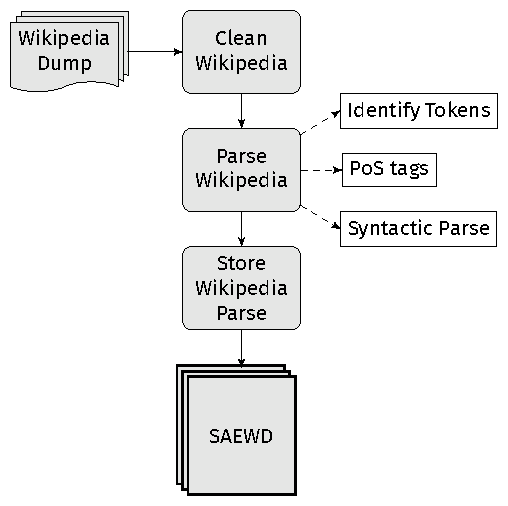
\includegraphics[scale=.8]{images/Chapitre7/flow_chart.pdf}
	\caption{The tree steps we took to build SAEWD.}
	\label{fig:flow}

\end{figure}

\subsection{Construction of SAEWD}
The three main steps we followed to build SAEWD are presented in Figure \ref{fig:flow}. Briefly, we have one input, which is the Wikipedia dump and one output which is the parsed snapshot. In the following we provide a detailed description of each of the process. 

 
We begin the construction of the parsed corpus with the Wikipedia dump XML file obtained from the Wikipedia database\footnote{\url{https://dumps.wikimedia.org/enwiki}} from early November 2014. This dump  contains around 4.7 million article pages\footnote{We kept all articles available in the Wikipedia dump.}. As shown in Figure \ref{fig:flow}, we apply the following processing steps in order to yield the final parsed version.
 
\subsubsection{Cleaning Wikipedia} First, we discard Wikipedia's  tables, references and lists, markup annotations and HTML tags with the \textit{WikiExtractor} \cite{Attardi2015}  script. 
We used this tool to clean and split the content of the original XML file into 429 folders each one containing 100 files of approximately 300 kB. These files contain a certain number of complete Wikipedia articles which is automatically determined by WikiExtractor  according to the maximum possible size assigned for each file, 300 kB in our case, thus the number of articles in each file may vary. We decided to use numerous files as well as a small size to easily read their content into memory while parsing. Having multiple small files also makes it easier to handle the multi-threading aspect of our parsing tool.
We kept WikiExtractor's original folder nomenclature which assigns to each one of them a sequence of letters sorted lexicographically\footnote{We have folders named \textit{AA}, \textit{AB}, \textit{AC} and so on.}. The files containing the cleaned text is simply named \textit{wiki\_XX} where  \textit{XX} goes from 00 to 99, as we have 100 files per folder. 
It is important to note that the Wikipedia articles' titles themselves are not sorted in any specific way, as it was not in the interest of our research to have them ordered. 
Inside each cleaned file, besides the article's text, WikiExtractor keeps the original article's URL as well as its unique Wikipedia ID within an XML-like label that also doubles as  article separator. 

\subsubsection{Parsing Wikipedia} Next, once the Wikipedia dump had been cleaned, we use the Stanford CoreNLP\footnote{\url{http://nlp.stanford.edu/software/corenlp.shtml}} \cite{manning2014} analysis tools to parse all the file texts produced during the previous step. As a part of our processing pipeline, we first perform  sentence segmentation, word tokenization and lemmatization. Below, we briefly describe each of the extracted attributes. We also exemplify them in detail in Section \ref{text:description}.
\begin{itemize}
\item PoS tagging: We obtain the grammatical category of each word, i.e., the part-of-speech tag, using the CoreNLP default tagger, the \textit{left3words} PoS tagging model.
\item Dependency parse: this attribute consists on an extracted tree that describes the types of grammatical relations between words, i.e., the dependency-based parse tree. 
The analysis was performed with the Stanford's \textit{Shift-Reduce}  parser.
% This parser is known to perform better than other Stanford parsers.                                  
 %(notably  faster and  with stronger \textit{F1} measure than the previous PCFG parser, although not as accurate as the Recurrent Neural Network system trained with semantic word vectors).
As information representation, we use the basic dependencies scheme, as we wanted to include each one of the possible dependency relations without any collapsing between them.    
                                                                                                                                                                                    
                                                                                                                                                                                    
\item Constituents parse:                                                                                                                                                           
the output of this analysis is a rooted tree that represents the syntactic structure of a phrase.                                                                                  
This tree is commonly known as the constituency-based parse tree.                                                                                                                  
For each word, we store its complete path in the constituency tree.
 Specifically, we keep all the nodes of a word's own branch from the root to the word itself.
 We employ the Stanford Shift-Reduce parser.
 This path is transformed into a single line and included in SAEWD. 
 

\end{itemize} 	
%\subsection{Parsed files organization}
 Finally, once the parsing process is complete, the parsed files are stored into individual files and thus there are as much parsed files as input Wikipedia cleaned files. The parsed files keep their original name plus the \texttt{parsed} extension, e.g., \texttt{wiki\_00.parsed}. The structure within the files is described in Section \ref{section3.2}. After parsing, we found the statistics shown in Table \ref{tab:corpus_stats}.
 
\begin{table}[t]
\centering
\caption{English Wikipedia dump statistics.}
\label{tab:corpus_stats}
\begin{tabular}{lr}
{\bf Number of tokens}      & 1,889,769,908 \\
{\bf Unique tokens (types)} & 8,761,691 \\
{\bf Number of sentences}   &  84,760,512\\
{\bf Average number of tokens per sentence} & 22.30
\end{tabular}
\end{table}

\subsection{SAEWD Description}\label{text:description}
In this section we describe in detail the characteristics of SAEWD.




\begin{table*}[ht]
\centering
\caption{Extract of a Wikipedia parsed file. The phrase shown is the parse result of the previous example sentence in Figure~\ref{fig:tree} }
\label{tab:parse}
\noindent\makebox[\textwidth]{%
\begin{tabular}{llllll}
 \multicolumn{6}{l}{\textit{FILENAME wiki\_00.parsed}}                                           \\ \hline
  \textbf{token}   & \textbf{lemma}   & \textbf{POS} & \textbf{constituency}                      & \textbf{head} & \textbf{dependency} \\ \hline
 \multicolumn{6}{l}{\textit{\%\%\#PAGE Anarchism}}                                         \\ \hline
  {$\vdots$}      &      {$\vdots$}   &  {$\vdots$}   &     {$\vdots$}                              &    {$\vdots$}  &     {$\vdots$}       \\  \hline
 \multicolumn{6}{l}{\textit{\%\%\#SEN 25  9}}                                             \\ \hline
						 A       & a       & DT  & NP\_22,S\_97                      & 3    & det        \\ %\cline{2-7} 
                         great   & great   & JJ  & NP\_22,S\_97                      & 3    & amod       \\ %\cline{2-7} 
                         brigand & brigand & NN  & NP\_22,S\_97                      & 4    & nsubj      \\ %\cline{2-7} 
                         becomes & become  & VBZ & VP\_44,S\_97                      & 0    & root       \\ %\cline{2-7} 
                         a       & a       & DT  & NP\_18,NP\_20,VP\_44,S\_97        & 6    & det        \\ %\cline{2-7} 
                         ruler   & ruler   & NN  & NP\_18,NP\_20,VP\_44,S\_97        & 4    & xcomp      \\ %\cline{2-7} 
                         of      & of      & IN  & PP\_57,NP\_20,VP\_44,S\_97        & 9    & case       \\ %\cline{2-7} 
                         a       & a       & DT  & NP\_18,PP\_57,NP\_20,VP\_44,S\_97 & 9    & det        \\ %\cline{2-7} 
                         Nation  & nation  & NN  & NP\_18,PP\_57,NP\_20,VP\_44,S\_97 & 6    & nmod       \\ %	\cline{2-7} 
\hline 
      
\end{tabular}}
\end{table*}

% Please add the following required packages to your document preamble:
% \usepackage{multirow}
% \usepackage{graphicx}
\begin{table*}[ht]
\centering
\resizebox{\textwidth}{!}{%
\begin{tabular}{cl|cccc|cccc|c}
\multirow{2}{*}{\textbf{PoS Tag}} & \multirow{2}{*}{\textbf{Token}} & \multicolumn{4}{c}{\textbf{NP}} & \multicolumn{4}{c}{\textbf{DEP}} & \multicolumn{1}{l}{\textbf{SEN}} \\ 
 &  & \multicolumn{1}{c}{$ \text{NP\_22}_1 $} & \multicolumn{1}{c}{$ \text{NP\_20}_1 $} & $ \text{NP\_18}_1  $& \multicolumn{1}{c}{$ \text{NP\_18}_2 $} & nsubj\_become & xcomp\_become & nmod\_ruler & \multicolumn{1}{c}{amod\_brigand} & \multicolumn{1}{l}{$ \text{~~S}_1 $} \\ \cline{1-11} 
\multirow{3}{*}{\textbf{NN}} & \multicolumn{1}{l|}{brigand} & 1 &  &  &  & 1 &  &  & & 1 \\
 & \multicolumn{1}{l|}{ruler} &  & 1 & 1 &  &  & 1 &  &  & 1 \\
 & \multicolumn{1}{l|}{nation} &  & 1 &  & 1&  &  & 1 &  & 1 \\ \hline
\textbf{VB} & \multicolumn{1}{l|}{becomes} &  &  &  &  &  &  &  & & 1 \\ \hline
\textbf{JJ} & \multicolumn{1}{l|}{great} & 1 &  &  &  &  &  &  & 1 & 1 \\ \hline
\end{tabular}
}
\caption{Brief example of the linguistic network incidence matrix of the previous used phrase. On the left side, as on the top, we can see the metadata we store for each word (rows) and each column (hyperedges). We omit the rest of the words from the example phrase for brevity.  }
\label{ref:incidence}
\end{table*}

\subsubsection{Constituency parse storage in detail}
%The  result from the constituency parse is not as straightforward to store as the other kinds of parses, i.e., the output is  a deeper tree structure than that of a dependency parse. Thus, we believe that the storage of this information in SAEWD requires a more in detail explanation. 
%In this subsection, we will describe how we stock the information concerning  the phrases' constituents. 

We will use an example to better explain the storage of the constituency-based parse tree. In Figure \ref{fig:tree} we can see the constituency parse of the phrase  \textit{A great brigand becomes a ruler of a Nation}. On the bottom of the figure, we observe the constituent's path (or branch), of the words \textit{brigand} and \textit{Nation}. As in any tree structure, each leaf node has a defined path from the root node to itself. In this example, the leaf containing the noun \textit{brigand} 
%(PoS tag \textit{NN})
 follows the bottom-up path \textit{NP22}$\rightarrow$\textit{S97}. \textit{Brigand's} parent node is a Noun Phrase (NP) node which in turn comes from the root of the tree, the Sentence node \textit{S}. We assign to each phrase chunk an identifier (22 and 97 in this case) in order to distinguish them according to their building elements as specified by the grammar rule used.
  In other words, a phrase chunk, e.g., a NP, a Verbal Phrase (VP), a Prepositional Phrase (PP), or other chunk defined by the grammar in CoreNLP, may be built from different types of PoS tags. Thus, again from Figure \ref{fig:tree}, we see that the sentence \textit{S97} is  built both from a NP and a VP chunk. 
 In a similar way, the noun phrase \textit{NP18} is produced by a determinant (DT) and a noun (NN), while  \textit{NP22} is generated by a determinant, an adjective (JJ) and a noun.
  The identification digits are obtained from the hash code that represents each chunk object inside our Java application. For each phrase-chunk tree node, we keep the last two significative figures produced by the \texttt{hashCode}\footnote{Java \texttt{hashCode} function description: \url{https://en.wikipedia.org/wiki/Java\_hashCode\%28\%29}} Java method.

\forestset{
    sn edges/.style={for tree={parent anchor=south, child anchor=north}},
    blue text/.style={for tree={text=blue!70}}}

\begin{figure}[]
\resizebox{\linewidth}{!}{%
\begin{forest} 
[S97
	[NP22 [DT [A, blue text]] [JJ [great, blue text]] [NN [brigand, blue text]]]
    [VP44 [VBZ [becomes, blue text]]
      [NP20
        [NP18 [DT [a, blue text]] [NN [ruler, blue text]]]
        [PP57 [IN [of, blue text]]
          [NP18 [DT [a, blue text]] [NN [Nation, blue text]]]]]]]
	\node [draw,fill = blue!20,text width=21em] at (1.5,-6.8) (sparse) {\textbf{brigand} (NN): NP22$\rightarrow$S97 \\ \textbf{Nation} (NN): NP18$\rightarrow$PP57$\rightarrow$NP20$\rightarrow$VP44$\rightarrow$S97};
\end{forest}
}

\caption{Constituency tree for the phrase \textit{{A great brigand becomes a ruler of a Nation}.}
% On the bottom, we can see the bottom-up path stored for the words \textit{brigand} and \textit{Nation}.
}
\label{fig:tree}
\end{figure}

 


As another example, the noun \textit{Nation} has the following bottom-up constituency path: \textit{NP18}$\rightarrow$\textit{PP57}$\rightarrow$\textit{NP20}$\rightarrow $\textit{VP44}. Indeed, the string \texttt{NP\_18,PP\_57,NP\_20,VP\_44,S\_97}, originating from the previously described path,  is the information we keep about the constituency parse for each token in the Wikipedia dump.



\subsubsection{Annotation scheme}\label{section3.2}
To store the parsed text we use a scheme  inspired by that used in \cite{ATSERIAS08}. The format can be considered as a regular tsv file (i.e., the entries are separated by tab spaces) with additional metadata tags. An extract from a parsed file can be observed in Table \ref{tab:parse}. 

The file includes two headers: the first one simply indicates the name of the current parse file; the second one contains the names that describe each column. The tags and columns our parsed dump contains are the following:
\begin{itemize}
\item Metadata tags:
\begin{enumerate}
\item {FILENAME}: indicates the original file used to extract the current parse, 
\item {\%\%\#PAGE}: denotes a new Wikipedia article, as well as its title, 
\item {\%\%\#SEN}: marks the beginning of a new sentence. It is followed by two integers: (1) the number of the current sentence, and (2), the number of tokens in the sentence.

\end{enumerate}

\item Parse columns for each token:
\begin{enumerate}
\item Token: the token itself,
\item Lemma: the token the canonical form,
\item POS: its part of speech tag,
\item Constituency: the bottom-up constituency path described before,
\item Head: the head index of the dependency relation the current token belongs to,
\item Constituency: the name of the grammatical relationship this token participates in as a dependent.
\end{enumerate}
\end{itemize}

Using the example phrase introduced before (Table \ref{tab:parse}), the token \textit{becomes} has \textit{become} as lemma, it is a verb, thus it has \textit{VBZ} as PoS tag, its constituency path is \textit{VP\_44,S\_97}, so it belongs to the verb phrase {VP44} which in turn comes from sentence {S97}. Finally, \textit{becomes}, being the main verb, is in this case the grammatical root of the sentence and its head is by convention determined as  zero. 

Concerning the computation time, SAEWD takes around 40 hours to be produced using a general purpose laptop (Intel i7 4700MQ with 4 cores, 8 GB and Linux Mint 17 as operative system). Most of the time is taken by the parsing step. 

We verified the consistency of the corpus built by analyzing a sample of 20 Wikipedia articles. The output of CoreNLP and the information contained in the corpus match.



